%
% 
%
\chapter{Resultados e Discussões} \label{chap:resultados}

\section{Avaliação de Consistência dos Dados de Literatura}

Após a implementação da metodologia descrita no \autoref{chap:metodologia}, os
resultados encontrados foram significativamente diferentes daqueles apresentados
por \citeonline{Rojas2014a}. A figura \autoref{fig:perfilTvalidacao}, por
exemplo, compara o perfil de temperatura dos leitos reais (de planta) com os
resultados da simulação implementada por \citeonline{Rojas2014a} e com os
resultados do trabalho aqui apresentado.

\begin{figure}[htb]
\centering 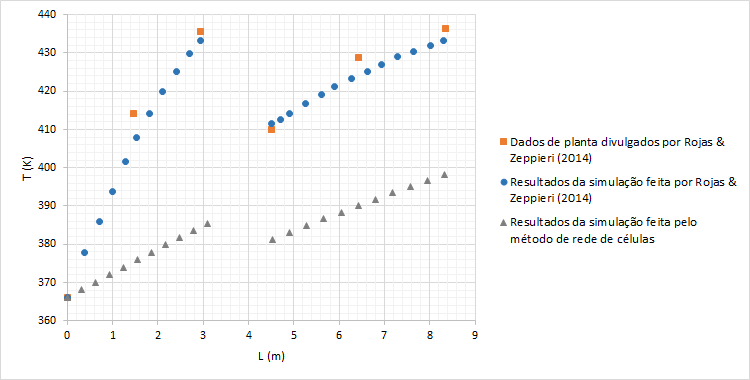
\includegraphics[scale=0.75]{images/Chap4/perfilTvalidacao.png}
\caption{Perfil de temperatura dos leitos}
\label{fig:perfilTvalidacao}
\end{figure}

Duas questões precisam ser destacadas da \autoref{fig:perfilTvalidacao}.
A primeira delas refere-se a exortermia dos leitos catalíticos: a modelagem aqui
desenvolvida apresenta exortemia inferior aos demais dados. Esse fato, quando
analisado isoladamente, induz ao pensamento de que ou a simulação
por rede de células não fora bem equacionada ou a abordagem é inadequada para o
sistema estudado.

A segunda questão refere-se ao resfriamento na região zona de \emph{quench}. O
dado de planta apresenta um resfriamento de $25,7 K$ entre os leitos
catalíticos; a simulação de \citeonline{Rojas2014a} apresenta resfriamento de
$21,6 K$ para a região; e o valor encontrado no presente trabalho foi de $4,1
K$. Essa situação torna-se mais enigmática ao se constatar que o balanço de
energia proposto por \citeonline{Rojas2014a} para a região de \emph{quench}
contém simplificações não realizadas neste estudo.

Uma análise do valor de LHSV (\emph{Liquid Hourly Space Velocity} foi feita
na tentativa de trazer um esclarecimento às discrepâncias encontradas. O
parâmetro LHSV pode ser definido como: 

\begin{equation}
LHSV = F_{vol}^L/{V_{R}}
\label{eq:LHSV}
\end{equation}

onde $F_{v}^L$ é a vazão volumétrica em $m^3/h$ de líquido e $V_{R}$ é o
volume total do reator (somando-se os dois leitos).

\nomenclature{$F_v$}{Vazão volumétrica \nomunit{m^3/h}}
\nomenclature[S]{$v$}{Referente à volume}
\nomenclature{$V$}{Volume \nomunit{m^3}}
\nomenclature{$V_R$}{Volume total do reator \nomunit{m^3}}

A \autoref{tab:comparacaoLHSV} mostra alguns valores encontrados na literatura
para LHSV, inclusive o valor para o trabalho de \citeonline{Rojas2014a}.

\begin{table}[!htb]
\begin{center}
\caption{Comparação entre LHSV publicados na literatura}
\label{tab:comparacaoLHSV}
\small
\begin{tabular}{lccc}
{Autor} & {$F_v^L$($m^3/h$)} & {$V_R$ ($m^3$)} &
{LHSV ($1/h$)}
\\
\hline
{\citeonline{Arpornwichanop2008}} & $69$ & $60$ & $1,14$ \\
{\citeonline{Mederos2007}} & $165$ & $62$ & $2,66$ \\
{\citeonline{Rojas2014a}} & $347$ & $18$ & $19,76$ \\
\bottomrule
\end{tabular}
\end{center}
\end{table}

Comparativamente, fica claro que o valor de LHSV do trabalho de
\citeonline{Rojas2014a} está uma ordem de grandeza acima dos valores
comumente empregados nos projetos de reatores TBR.

Sendo assim, foi necessário alterar o valor da vazão de alimentação de gasolina
de pirólise para que os dados apresentassem coerência. O critério
utilizado foi o resfriamento da região de \emph{quench}, já que essa seção do
reator é de baixa complexidade fenomenológica e, pelo rigor termodinâmico aqui
utilizado, deveria apresentar valor próximo ao dado de planta.

Após várias tentativas, o valor de $F_{w,1}$ foi alterado para $2,079.10^4
kg/h$. Com essa nova vazão o tanto o resfriamento da região de \emph{quench} quando a exotermia dos leitos tornaram-se aderentes aos
dados de planta e de literatura, como está descrito nas próximas seções.

A \autoref{tab:comparacaoLHSV2} repete os valores da
\autoref{tab:comparacaoLHSV}, mas agora com a inclusão do valor ajustado e que
foi usado neste trabalho.

\begin{table}[!htb]
\begin{center}
\caption{Comparação entre LHSV}
\label{tab:comparacaoLHSV2}
\small
\begin{tabular}{lccc}
{Autor} & {$F_v^L$ ($m^3/h$)} & {$V_R$ ($m^3$)} &
{LHSV ($1/h$)}
\\
\hline
{\citeonline{Arpornwichanop2008}} & $69$ & $60$ & $1,14$ \\
{\citeonline{Mederos2007}} & $165$ & $62$ & $2,66$ \\
{\citeonline{Rojas2014a}} & $347$ & $18$ & $19,76$ \\
{Valor ajustado} & $76$ & $18$ & $4,34$ \\
\bottomrule
\end{tabular}
\end{center}
\end{table}

\section{Estado Estacionário} \label{sec:estadoestacionario}

\section{Respostas Dinâmicas} \label{sec:respostasdinamicas}





























